\chapter{Model and Experiment settings}
\label{chapterlabel3}
In this chapter we will describe the seq2seq model\cite{sutskever2014sequence,cho2014learning} in detail, we also introduce different objective functions for training seq2seq model and evaluation metrics we will use to carry out our analysis.
\section{Sequence to Sequence Model}
Seq2seq model\cite{sutskever2014sequence,cho2014learning} emerges as an effective paradigm for dealing with variable length inputs and outputs.
The model consists of an encoding and a decoding RNNs, the encoding RNN processes input sequence $ \{\mathbf{x_{1:n}}\}$ to emit a fixed size context vector $\mathbf{c}$. 
Then the decoding RNN generate a output sequence conditional on the context vector $\mathbf{c}$\cite{Goodfellow2016Book}.
\subsection{Encoding RNN}
We first feed input sentence $\mathbf{x_{1:n}}$ to a bidirectional RNN\cite{schuster1997bidirectional} with GRU\cite{chung2014empirical} to obtain forward information $\overrightarrow{\mathbf{h}}_{1:n}$ and backward information $\overleftarrow{\mathbf{h}}_{1:n}$:
\begin{equation}
\overrightarrow{\mathbf{h}}_{i} =\begin{cases}
(1-\overrightarrow{\mathbf{z}}_{i})\odot\overrightarrow{\mathbf{h}}_{i-1} + \overrightarrow{\mathbf{z}}_{i}\odot\overrightarrow{\mathbf{h}}'_{i} & \text{if i \textgreater 0}\\
0 & otherwise \\
\end{cases}
\end{equation}
Where
\begin{equation}
\overrightarrow{\mathbf{h_{i}}'} = \tanh(\overrightarrow{\mathbf{W}}\mathbf{x}_{i}+\overrightarrow{\mathbf{U}}\begin{bmatrix}
	\overrightarrow{\mathbf{r}}_{i}\odot\overrightarrow{\mathbf{h}}_{i-1}
	\end{bmatrix})
\end{equation}
\begin{equation}
\overrightarrow{\mathbf{z}}_{i} = \sigma(\overrightarrow{\mathbf{W}}_{z}\mathbf{x_{i}}+\overrightarrow{\mathbf{U}}_{z}\overrightarrow{\mathbf{h}}_{i-1})
\end{equation}
\begin{equation}
\overrightarrow{\mathbf{r}}_{i}= \sigma(\overrightarrow{\mathbf{W}}_{r}\mathbf{x_{i}}+\overrightarrow{\mathbf{U}}_{r}\overrightarrow{\mathbf{h}}_{i-1})
\end{equation}
$\overrightarrow{\mathbf{W}},\overrightarrow{\mathbf{W}}_{z},\overrightarrow{\mathbf{W}}_{r}$ and  $\overrightarrow{\mathbf{U}},\overrightarrow{\mathbf{U}}_{z},\overrightarrow{\mathbf{U}}_{r}$ are weight matrices, $\sigma(\cdot)$ is a sigmoid function. 
Note that the backward hidden states are computed similarly, with different sets of weight matrices. 
The outputs of bidirectional RNN is the concatenate of forward and backward information.
\begin{equation}
\mathbf{h_{i}} = \begin{bmatrix}
\overrightarrow{\mathbf{h}}_{i} \\
\overleftarrow{\mathbf{h}}_{i}\\
\end{bmatrix}
\end{equation}
The $\mathbf{h_{1:n}}$ are encoded by another RNN with GRU, and we take the final output of this RNN as the fixed context representation $\mathbf{c}$ of input sentence.
\subsection{Decoding RNN}
The decoding RNN computes outputs $\mathbf{s}_{1:m}$ as following
\begin{equation}
\mathbf{s_{j}} =\begin{cases}
(1-\mathbf{z_{j}})\odot\mathbf{s_{j-1}} + \mathbf{z_{j}}\odot \mathbf{\bar{s_{j}}} & \text{j \textgreater 0}\\
0 & \text{otherwise}\\
\end{cases} 
\end{equation}
Where $\mathbf{s}_{j}$ is calculated conditional on $\mathbf{c}$
\begin{equation}
\mathbf{\bar{s_{j}}} = \tanh(\mathbf{Wx_{j-1}}+\mathbf{r_{j}}\odot\begin{bmatrix}
\mathbf{Us_{j-1}}+\mathbf{Vc}
\end{bmatrix})
\end{equation}
\begin{equation}
\mathbf{z_{j}} = \sigma(\mathbf{W_{z}x_{j-1}}+\mathbf{U_{z}s_{j-1}}+\mathbf{V_{z}c})
\end{equation}
\begin{equation}
\mathbf{r_{j}} = \sigma(\mathbf{W_{r}x_{j-1}}+\mathbf{U_{r}s_{j-1}}+\mathbf{V_{r}c})
\end{equation}
Then with the target output sequence $\mathbf{y}_{1:m}$, we can compute the output conditional probability\cite{cho2014learning}
\begin{equation}
p_{\mathbf{\theta}}(\mathbf{y}_{1:m}|\mathbf{x_{1:n}}) = \prod_{j=1}^{m} p_{\mathbf{\theta}}(\mathbf{y}_{j}|\mathbf{y}_{j-1},\mathbf{c})
\end{equation} 
\begin{equation}
p_{\mathbf{\theta}}(\mathbf{y}_{j}|\mathbf{y}_{j-1},\mathbf{c}) = \frac{\exp(\mathbf{y}_{j}^{T}\mathbf{W_{p}e_{j}} )}{\sum_{\mathbf{y}_{k} \in \mathbf{{V}}}\exp(\mathbf{y}_{k}^{T}\mathbf{W_{p}e_{i}})}
\end{equation}
\begin{equation}
\mathbf{e_{i}} = \mathbf{O_{e}s_{i-1}} + \mathbf{O_{y}y_{i-1}} + \mathbf{O_{c}c}
\end{equation}
Where $\mathbf{\theta}$ indicate all the parameters of our seq2seq model, $\mathbf{{V}}$ is feature vectors of full vocabulary set. The negative log likelihood is considered as the loss function of seq2seq model
\begin{equation}\label{eq:seq2seq-loss}
L_{rec} = -\sum_{j=1}^{m}\log p_{\mathbf{\theta}}(\mathbf{y}_{j}|\mathbf{y}_{j-1},\mathbf{c})
\end{equation}
\begin{figure*}[h!]
	\centering
	\def\layersep{2.5cm}
	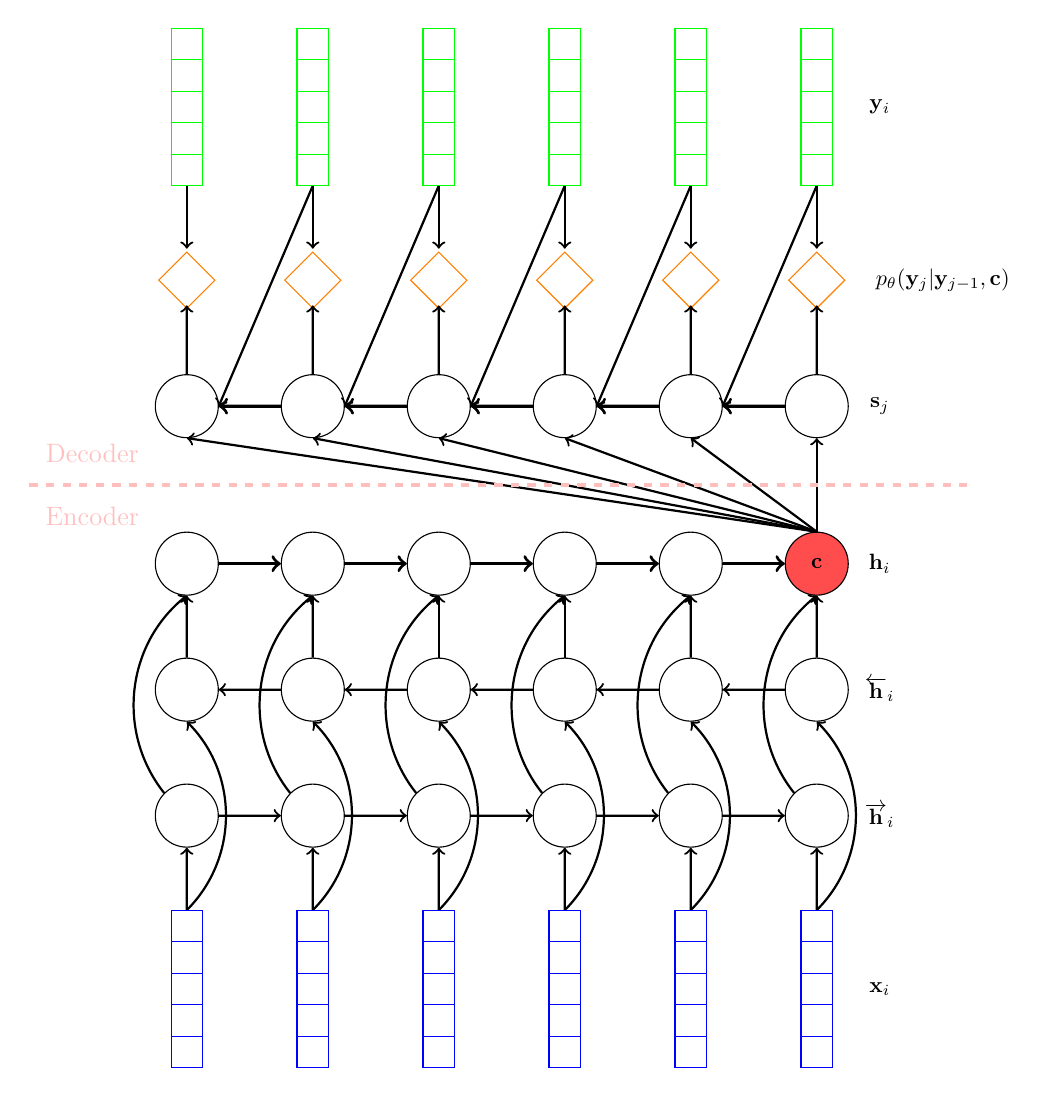
\begin{tikzpicture}[node distance = \layersep,scale=0.8, every node/.style={scale=0.8}]
	\tikzstyle{neuron} = [circle,minimum size=1cm]
	\tikzstyle{prob} = [rectangle, minimum height=0.63cm,minimum width=0.63cm]
	\tikzstyle{ks} = [rectangle,minimum height=0.5cm,minimum width=0.5cm]
	
	
	\node[draw=orange,prob,rotate=45](p-1) at (-5,4.5){};
	\node[draw=orange,prob,rotate=45](p-2)at (-3,4.5){};
	\node[draw=orange,prob,rotate=45](p-3)at (-1,4.5){};
	\node[draw=orange,prob,rotate=45](p-4)at (1,4.5){};
	\node[draw=orange,prob,rotate=45](p-5)at (3,4.5){};
	\node[draw=orange,prob,rotate=45](p-6)at (5,4.5){};
	
	
	\node[draw,neuron](d-1)at(-5,2.5){};
	\node[draw,neuron](d-2)at(-3,2.5){};
	\node[draw,neuron](d-3)at(-1,2.5){};
	\node[draw,neuron](d-4)at(1,2.5){};
	\node[draw,neuron](d-5)at(3,2.5){};
	\node[draw,neuron](d-6)at(5,2.5){};
	
	\path[->,very thick] (d-6) edge (d-5)
	(d-5) edge (d-4)
	(d-4) edge (d-3)
	(d-3) edge (d-2)
	(d-2) edge (d-1);
	
	\node[draw,neuron](e-1)at(-5,0){};
	\node[draw,neuron](e-2)at(-3,0){};
	\node[draw,neuron](e-3)at(-1,0){};
	\node[draw,neuron](e-4)at(1,0){};
	\node[draw,neuron](e-5)at(3,0){};
	\node[draw,neuron,fill=red!70](e-6)at(5,0){$\mathbf{c}$};
	
	\path[->,very thick] (e-1) edge (e-2)
	(e-2) edge (e-3)
	(e-3) edge (e-4)
	(e-4) edge (e-5)
	(e-5) edge (e-6);
	
	\node[draw,neuron](b-1)at(-5,-2){};
	\node[draw,neuron](b-2)at(-3,-2){};
	\node[draw,neuron](b-3)at(-1,-2){};
	\node[draw,neuron](b-4)at(1,-2){};
	\node[draw,neuron](b-5)at(3,-2){};
	\node[draw,neuron](b-6)at(5,-2){};
	
	\path[->,thick] (b-6) edge (b-5)
	(b-5) edge (b-4)
	(b-4) edge (b-3)
	(b-3) edge (b-2)
	(b-2) edge (b-1);
	
	
	
	\node[draw,neuron](f-1)at(-5,-4){};
	\node[draw,neuron](f-2)at(-3,-4){};
	\node[draw,neuron](f-3)at(-1,-4){};
	\node[draw,neuron](f-4)at(1,-4){};
	\node[draw,neuron](f-5)at(3,-4){};
	\node[draw,neuron](f-6)at(5,-4){};
	
	\path[->,thick] (f-1) edge (f-2)
	(f-2) edge (f-3)
	(f-3) edge (f-4)
	(f-4) edge (f-5)
	(f-5) edge (f-6);
	
	\foreach \i in {1,...,6}{
		\path[->,thick] (b-\i) edge (e-\i);
		\path[->,thick, bend left=45] (f-\i) edge (e-\i.south);
		\path[->,thick] (e-6.north) edge (d-\i.south);
	};
	
	\path[->,thick] (-5,-5.5) edge (f-1.south)
	(-3,-5.5) edge (f-2.south)
	(-1,-5.5) edge (f-3.south)
	(1,-5.5) edge (f-4.south)
	(3,-5.5) edge (f-5.south)
	(5,-5.5) edge (f-6.south);
	
	\path[->,thick] (d-1) edge (-5,4.1)
	(d-2) edge (-3,4.1)
	(d-3) edge (-1,4.1)
	(d-4) edge (1,4.1)
	(d-5) edge (3,4.1)
	(d-6) edge (5,4.1);
	
	\path[->,thick,bend right=45] (-5,-5.5) edge (b-1.south)
	(-3,-5.5) edge (b-2.south)
	(-1,-5.5) edge (b-3.south)
	(1,-5.5) edge (b-4.south)
	(3,-5.5) edge (b-5.south)
	(5,-5.5) edge (b-6.south);
	
	\path[->,thick] (-5,6) edge (-5,5)
	(-3,6) edge (-3,5)
	(-1,6) edge (-1,5)
	(1,6) edge (1,5)
	(3,6) edge (3,5)
	(5,6) edge (5,5);
	
	\path[->,thick](-3,6) edge (d-1.east)
	(-1,6) edge (d-2.east)
	(1,6) edge (d-3.east)
	(3,6) edge (d-4.east)
	(5,6) edge (d-5.east);
	
	\foreach \j in {-5,-3,-1,1,3,5}{
		\foreach \i in {1,...,5}{
			\node[draw=blue,ks] at (\j,-5.25-\i*0.5){};
			\node[draw=green,ks] at (\j,5.75+\i*0.5){};
		};	
	};
	
	\node[](hf) at (6,-4) {$\overrightarrow{\mathbf{h}}_{i}$};
	\node[](hb) at (6,-2) {$\overleftarrow{\mathbf{h}}_{i}$};
	\node[](h) at (6,0){$\mathbf{h}_{i}$};
	\node[](d) at (6,2.5){$\mathbf{s}_{j}$};
	\node[](p) at (7,4.5) {$p_{\mathbf{\theta}}(\mathbf{y}_{j}|\mathbf{y}_{j-1},\mathbf{c})$};
	\node[](x)at(6,-6.75) {$\mathbf{x}_{i}$};
	\node[](y)at(6,7.25) {$\mathbf{y}_{i}$};
	\draw[very thick, dashed,pink]{(-7.5,1.25) -- (7.5,1.25)};
	\node[]()at(-6.5,0.75){\large{\textcolor{pink}{Encoder}}};
	\node[]()at(-6.5,1.75){\large{\textcolor{pink}{Decoder}}};
	\end{tikzpicture}
	\caption{Seq2seq model with bidirectional RNN encoder \cite{cho2014learning}, the input word feature vectors are first encoded by a bidirectional RNN into fixed context vector $\mathbf{c}$,then the decoder calculate the probability of decoding sequence conditional on this context vector $\mathbf{c}$.}
\end{figure*}
\section{Loss Estimation}
Training the seq2seq on large vocabulary can incur the problem of intractable computation\cite{cho2015using}. Let us consider the gradient of Equation \ref{eq:seq2seq-loss}. For convenient we let $f_{\mathbf{\theta}}(\mathbf{y},\mathbf{e}) = \mathbf{y}^{T}\mathbf{W_{p}}\mathbf{e} $ ,the gradient can be composed as follow:
\begin{equation}\label{softmax_g}
g_{\mathbf{\theta}} = \bigtriangledown_{\mathbf{\theta}}f_{\mathbf{\theta}}(\mathbf{y_{j},e_{j}}) -\sum_{\mathbf{y_{k}\in V}} \frac{\exp(f_{\mathbf{\theta}}(\mathbf{y_{k},e_{j}}))}{Z}\bigtriangledown_{\mathbf{\theta}}f_{\mathbf{\theta}}(\mathbf{y_{k},\mathbf{e}_{j}})
\end{equation}
Where $Z = \sum_{\mathbf{y_{k}\in \mathbf{{V}}}}\exp(f_{\mathbf{\theta}}(\mathbf{y_{k},e_{j}}))$. 
When the size of $\mathbf{{V}}$ becomes large, the normaliser $Z$ quickly becomes intractable\cite{bengio2003quick}. 
A common way to address this issue is to approximate this term by importance sampling\cite{murphy2012machine}: 
\begin{equation}
Z = \sum_{\mathbf{y_{k}\in \mathbf{{V}}}}q(\mathbf{y_{k}})\frac{\exp(f_{\mathbf{\theta}}(\mathbf{y_{k},e_{j}}))}{q(\mathbf{y_{k}})} \approx \frac{1}{S}\sum_{s=1}^{S}\frac{\exp(f_{\mathbf{\theta}}(\mathbf{y_{s},e_{j}}))}{q(\mathbf{y_{s}})}
\end{equation}
Where $\mathbf{y}_{s}$ is the sample drawn from the proposed importance distribution $q(\mathbf{y})$. We can predefine a small subset of vocabulary $\mathbf{{V}}_{s} \subset \mathbf{{V}}$ with size $s$, and assume the distribution  $q(\mathbf{y})$ has the form\cite{bengio2008adaptive}:
\begin{equation}
q(\mathbf{y}) = \begin{cases}
\frac{1}{S} & \text{if } \mathbf{y} \in \mathbf{{V}}_{s} \\
0 & \text{otherwise}
\end{cases}
\end{equation}
Under this assumption we can compute an approximated normalizer:
\begin{equation}
Z \approx \sum_{s=1}^{S}\exp(f_{\mathbf{\theta}}(\mathbf{y_{s},e_{j}}))
\end{equation}
By using this approach, we can estimate the value of both gradient $g_{\mathbf{\theta}}$ and likelihood function $p_{\mathbf{\theta}}\mathbf{(y_{j}|y_{j-1},c)}$ with a smaller subset of $\mathbf{{V}_{s}}$.
Which can reduce the computational cost during training.
\section{Finding the Prediction}
Unlike training time the target output sequences are available to model, at testing time seq2seq model must be able to predict the appropriate output sequences\cite{sutskever2014sequence}, this can be done via
\begin{equation}
\hat{\mathbf{y}}_{1:m} = \arg\max_{\mathbf{y_{1:m}} \in \mathbf{{V}}} p(\mathbf{y_{1:m}}|\mathbf{x_{1:n}}) = \arg\max_{\mathbf{y_{1:m}}\in \mathbf{{V}}} \prod_{t=1}^{m}p(\mathbf{y_{t}}|\mathbf{y_{t-1}},\mathbf{c})
\end{equation}
Viterbi algorithm can solve this problem with $O(m\times |\mathbf{{V}}|^{2})$ complexity\cite{viterbi1967error}
\begin{equation}
\alpha(\mathbf{y}_{0}) = 1
\end{equation}
\begin{equation}\label{Viterbi}
\alpha(\mathbf{y}_{t}) = \max_{\mathbf{y}_{t-1}\in\mathbf{{V}}}\alpha(\mathbf{y}_{t-1})p(\mathbf{y}_{t}|\mathbf{y}_{t-1},\mathbf{c})
\end{equation}
But with the size of vocabularies grows, the computational cost for decoding will become very expensive.
A much efficient approach is to apply Beam search with Viterbi decoder\cite{koehn2009statistical}. 
\begin{figure*}[h]
	\centering
	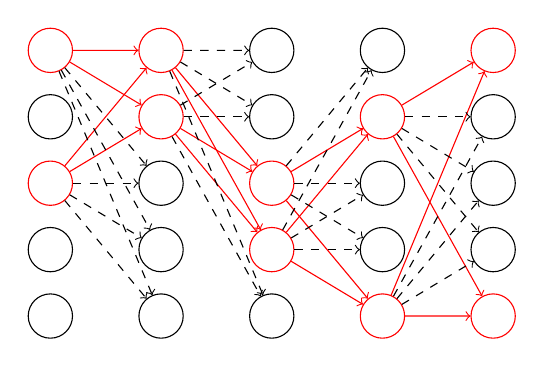
\begin{tikzpicture}[scale=0.8, every node/.style={scale=0.8}]
	\tikzstyle{active} = [circle,draw=red,minimum size = 2em]
	\tikzstyle{dump} = [circle,draw=black!100,minimum size = 2em]
	\node[active](a-1-1)at (-12em,7em){};
	\node[active](a-1-2)at (-12em,1em){};
	\node[dump](d-1-1)at (-12em,4em){};
	\node[dump](d-1-2)at (-12em,-2em){};
	\node[dump](d-1-3)at (-12em,-5em){};
	
	\node[active](a-2-1)at (-7em,7em){};
	\node[active](a-2-2)at (-7em,4em){};
	\node[dump](d-2-1)at (-7em,1em){};
	\node[dump](d-2-2)at (-7em,-2em){};
	\node[dump](d-2-3)at (-7em,-5em){};
	
	\node[active](a-3-1)at (-2em,-2em){};
	\node[active](a-3-2)at (-2em,1em){};
	\node[dump](d-3-1)at (-2em,7em){};
	\node[dump](d-3-2)at (-2em,4em){};
	\node[dump](d-3-3)at (-2em,-5em){};
	
	\node[active](a-4-1)at (3em,-5em){};
	\node[active](a-4-2)at (3em,4em){};
	\node[dump](d-4-1)at (3em,7em){};
	\node[dump](d-4-2)at (3em,-2em){};
	\node[dump](d-4-3)at (3em,1em){};
	
	\node[active](a-5-1)at (8em,7em){};
	\node[active](a-5-2)at (8em,-5em){};
	\node[dump](d-5-1)at (8em,1em){};
	\node[dump](d-5-2)at (8em,4em){};
	\node[dump](d-5-3)at (8em,-2em){};
	
	\path[color=red,->] (a-1-1) edge (a-2-1)
	(a-1-1) edge (a-2-2)
	(a-1-2) edge (a-2-1)
	(a-1-2) edge (a-2-2)
	(a-2-1) edge (a-3-1)
	(a-2-1) edge (a-3-2)
	(a-2-2) edge (a-3-1)
	(a-2-2) edge (a-3-2)
	(a-3-1) edge (a-4-1)
	(a-3-1) edge (a-4-2)
	(a-3-2) edge (a-4-1)
	(a-3-2) edge (a-4-2)
	(a-4-1) edge (a-5-2)
	(a-4-1) edge (a-5-1)
	(a-4-2) edge (a-5-1)
	(a-4-2) edge (a-5-2);
	\path[dashed,->] (a-1-1) edge (d-2-1)
	(a-1-1) edge (d-2-2)
	(a-1-2) edge (d-2-1)
	(a-1-2) edge (d-2-2)
	(a-2-1) edge (d-3-1)
	(a-2-1) edge (d-3-2)
	(a-2-2) edge (d-3-1)
	(a-2-2) edge (d-3-2)
	(a-3-1) edge (d-4-1)
	(a-3-1) edge (d-4-2)
	(a-3-2) edge (d-4-1)
	(a-3-2) edge (d-4-2)
	(a-4-1) edge (d-5-2)
	(a-4-1) edge (d-5-1)
	(a-4-2) edge (d-5-1)
	(a-4-2) edge (d-5-2);
	
	\path[dashed,->] (a-1-1) edge (d-2-3)
	(a-1-2) edge (d-2-3)
	(a-2-1) edge (d-3-3)
	(a-2-2) edge (d-3-3)
	(a-3-1) edge (d-4-3)
	(a-3-2) edge (d-4-3)
	(a-4-1) edge (d-5-3)
	(a-4-2) edge (d-5-3);
	
	\end{tikzpicture}
	\caption{Viterbi algorithm with Beam search with $k=2$. Only top 2 paths are kept in candidate set are explored (indicate by red color), other paths are discarded (indicate by dashed line).}
	\label{beam}
\end{figure*}

\noindent
Beam search is a heuristic search algorithm, which explores the search space by expanding a set of most promising candidates with size $k$\cite{russell2003artificial}. 
In our application is to rank all alternative candidate words at each time point and store top $k$ words in candidate set $\mathbf{V}_{k}$ for next evaluation.  
This changes Equation \ref{Viterbi} the original Viterbi algorithm to  
\begin{equation}
\alpha(\mathbf{y}_{t}) \approx \max_{\mathbf{y}_{t-1}\in\mathbf{{V}}_{k}}\alpha(\mathbf{y}_{t-1})p(\mathbf{y}_{t}|\mathbf{y}_{t-1},\mathbf{c})
\end{equation}
Figure \ref{beam} shows an example of Viterbi algorithm with Beam search applied.\\\\
The Viterbi Beam decoding can solve the problem with $O(m\times k \times |\mathbf{{V}}|)$ complexity. 
And the most probable sequence can be compute by backtracking. 
However beam search may not be able to find the best output sequences, as the vocabularies are not fully searched at each time steps. 
So there is always a trade off between the beam search efficiency and accuracy. 
For the sequence to sequence model, Sutskever et al \cite{sutskever2014sequence} suggested a beam size of 2 suffices to provide most of benefits of beam search.

\section{Objective Functions}
Here we introduce different objective functions used to train our seq2seq models.

\subsection{Unsupervised Pretrain}
We feed seq2seq model with English sentences and ask it to reconstruct input sentences as its output. 
This objective function is proposed by Dai et al \cite{dai2015semi}.
\begin{figure*}[h]
	\centering
	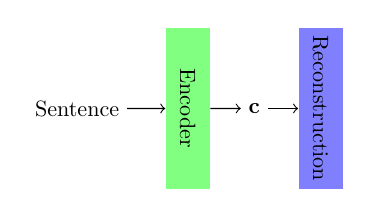
\begin{tikzpicture}[scale=0.8, every node/.style={scale=0.8}]
	\tikzstyle{block} = [rectangle,minimum width=7.3em,minimum height=2em]
	\node[block,fill=blue!50,rotate=270](reconstruction)at(6em,0em){Reconstruction};
	\node[block,fill=green!50,rotate=270](Encoder)at (0em,0){Encoder};
	\node[](s)at (-5em,0){Sentence};
	\node[](c)at(3em,0){$\mathbf{c}$};
	\path[->] (s) edge (Encoder)
	(Encoder) edge (c);
	\path[->] (c) edge (reconstruction.south);
	\end{tikzpicture}
	\caption{Unsupervised pretrain of seq2seq model. The seq2seq model is asked to reconstruction the input sentence as its output.}
\end{figure*}
\subsection{Semi Supervised Pretrain}
In language recognition, some pairs of sentences $(\mathbf{x_{1:n}},\mathbf{\bar{x}_{1:m}})$ with different expression might have similar meaning. 
This means, their learnt internal fixed context representation $(\mathbf{c},\mathbf{\bar{c}})$ suppose to be close under some measurements. \\\\
We provide a limited set of sentence's pairs with similar meaning to sequential autoencoder, and we define a constrained loss $L'$ as
\begin{equation}
L' =(\mathbf{c}-\bar{\mathbf{c}})^{T}(\mathbf{c}-\bar{\mathbf{c}})
\end{equation}
Therefore the overall loss $L$ of this setting is
\begin{equation}
L = \alpha L_{rec} + L' 
\end{equation}
Where $\alpha L_{rec}$ is the penalised reconstruction loss. 
Zhang et al \cite{zhang2014bilingually} try the similar idea with hinge loss on REA in machine translation, their observations show that the additional constraint can help model to learn closer representations for sentences with similar meaning. 
\begin{figure*}[h]
	\centering
	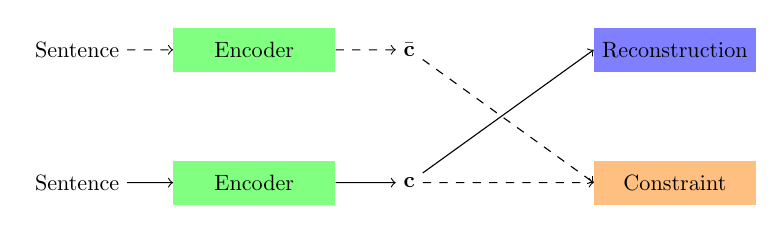
\begin{tikzpicture}[scale=0.8, every node/.style={scale=0.8}]
	\tikzstyle{block} = [rectangle,minimum width=7.3em,minimum height=2em]
	\node[block,fill=blue!50](reconstruction)at(13em,3em){Reconstruction};
	\node[block,fill=green!50](Encoder)at (-6em,-3em){Encoder};
	\node[block,fill=green!50](Encoder-c)at (-6em,3em){Encoder};
	\node[block,fill=orange!50](constraint)at (13em,-3em) {Constraint};
	\node[](s)at (-14em,-3em){Sentence};
	\node[](con)at (-14em,3em){Sentence};
	\node[](c)at(1em,-3em){$\mathbf{c}$};
	\node[](cc)at(1em,3em){$\bar{\mathbf{c}}$};
	\path[->] (s) edge (Encoder)
	(Encoder.east) edge (c);
	\path[dashed,->] (c) edge (constraint.west)
	(cc) edge (constraint.west)
	(Encoder-c) edge (cc)
	(con) edge (Encoder-c);
	\path[->]
	(c) edge (reconstruction.west);
	\end{tikzpicture}
	\caption{Semi supervised pretrain, the model is pretrained with constraint (indicate by dashed line).}
\end{figure*}
\subsection{Multiple Tasks Joint Training}
\begin{figure*}[h]
	\centering
	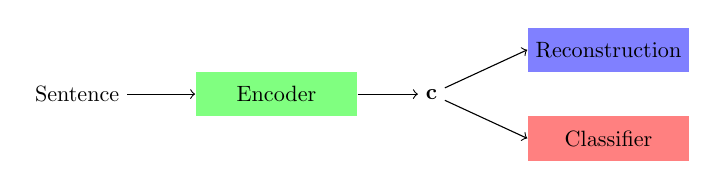
\begin{tikzpicture}[scale=0.8, every node/.style={scale=0.8}]
	\tikzstyle{block} = [rectangle,minimum width=7.3em,minimum height=2em]
	\node[block,fill=blue!50](reconstruction)at(12em,2em){Reconstruction};
	\node[block,fill=green!50](Encoder)at (-3em,0){Encoder};
	\node[block,fill=red!50](Classifier)at(12em,-2em){Classifier};
	\node[](s)at (-12em,0){Sentence};
	\node[](c)at(4em,0){$\mathbf{c}$};
	\path[->] (s) edge (Encoder)
	(Encoder) edge (c)
	(c) edge (Classifier.west)
	(c) edge (reconstruction.west);
	\end{tikzpicture}
	\caption{ Joint training, seq2seq model is joint trained with another supervised task.}
\end{figure*}

\noindent
We joint train seq2seq model with another supervised task. 
In this thesis the candidate supervised task includes sentiment analysis, machine translation and sentence entailment. 
The training objective function is
\begin{equation}
L(\mathbf{X},Y) = L_{c}+\alpha L_{rec}
\end{equation}
Where $\alpha L_{rec}$ is the penalised reconstruction loss, $ L_{c}$ is the classification loss of the supervised task.
Dong et al \cite{dong2015multi} and Luong et al\cite{luong2015multi} show that, multi-task training allows information shares across tasks, which will benefit the testing time performance.
\section{Intrinsic Evaluation}
In NLP, the intrinsic evaluation metric is one which measures the quality of a model independent of any application\cite{jurafsky2000speech}. 
The intrinsic evaluation is easy to carry out and usually used as a quick check of language models. 
\subsection{Euclidean Distance}
We use Euclidean distance as one of the intrinsic metrics, to be more specific, we calculate the Euclidean distance between representations of some selected sentence pairs, to see whether the Euclidean distance is smaller for pairs with similar meaning compares with those pairs have opposite meaning. 
\subsection{Perplexity}
We also compute the perplexity\cite{brown1992estimate} of each experimental models, to evaluate how well they can assign probabilities to a sample prediction.
The perplexity is calculate by
\begin{equation}
\text{perplexity}(\mathbf{y}_{1:m}) = \sqrt[m]{\prod_{i=1}^{m}\frac{1}{p(\mathbf{y}_{i}|\mathbf{y}_{i-1},\mathbf{c})}} 
\end{equation} 
When calculate perplexity we clip the value of $p(\mathbf{y}_{i}|\mathbf{y}_{i-1},\mathbf{c})$ to be in between $[0.01,1]$, so the the perplexity is within $[1,100]$.
Usually better models have lower perplexity. 

\section{Extrinsic Evaluation}
Extrinsic evaluation is the evaluation on real tasks. 
To carry out this evaluation, we tune our pretrained RNN encoder on sentence entailment, sentiment analysis and machine translation. 
The testing time performance is taken as the extrinsic evaluation metrics.

\subsection{Binary Sentiment Analysis}
\begin{figure*}[h]
	\centering
	\usetikzlibrary{positioning}
	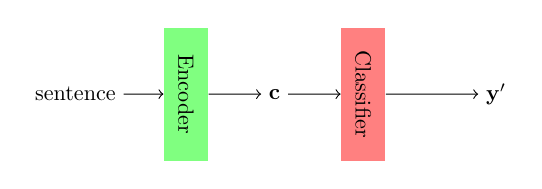
\begin{tikzpicture}[scale=0.8, every node/.style={scale=0.8}]
	\tikzstyle{block} = [rectangle,minimum width=6em,minimum height=2em]
	\node[rotate=270,block,fill=green!50]at (-15em,0)(encoder){Encoder};
	\node[](sentence)at (-20em,0){sentence};
	\node[](p)at (-1em,0){$\mathbf{y}'$};
	\node[rotate=270,block,fill=red!50](classifier)at (-7em,0){Classifier};
	\node[](c)at (-11em,0){$\mathbf{c}$};
	\path[->] (sentence) edge (encoder)
	(encoder)  edge (c)
	(c) edge (classifier)
	(classifier) edge (p);
	\end{tikzpicture}
	\caption{Sentiment analysis model, the sentence is first encoded into fixed context vector $\mathbf{c}$, and then pass to classifier to give predicted result $\mathbf{y}'$.}
\end{figure*}

\noindent
We pass the sentence representation $\mathbf{c}$ encoded by RNN encoder to a simple sigmoid binary classifier, 
\begin{equation}
p = \sigma(\mathbf{w}^{T}\mathbf{c}+b)
\end{equation}
We use cross entropy loss as objective function
\begin{equation}
L_{c} = ylog(p) + (1-y)log(1-p)
\end{equation}
At the testing time the prediction is given by
\begin{equation}
y' = \begin{cases}
0 &  p > 0.5 \\
1 &  p \leq 0.5 \\
\end{cases}
\end{equation}
Where 1 indicate positive sentiment, 0 indicate negative sentiment.
\subsection{Sentence Entailment}
In sentence entailment task, the model has to figure out whether the input sentence pair $\mathbf{X} = \{\mathbf{x_{1:n}^{p}},\mathbf{x_{1:m}^{h}}\}$ is entailed, natural or contradicted\cite{snli:emnlp2015}, these three relation are represent by different three dimensional one-hot vectors
\begin{align*}
\text{Entailment} = \begin{bmatrix}1 \\0 \\0 \\\end{bmatrix}& &
\text{Natural} = \begin{bmatrix}0 \\1 \\0 \\\end{bmatrix}& &
\text{Contradict} = \begin{bmatrix}0 \\0 \\1 \\\end{bmatrix}
\end{align*}
The output layer of sentence entailment task is designed as follow. After the RNN sentence encoder encodes the context vector $\mathbf{c_{p}}$ and $\mathbf{c_{h}}$ from the input pair, we construct a intermediate information vector $\mathbf{c_{ph}}$ by following the suggestion from\cite{mou2015recognizing}
\begin{equation}
\mathbf{c_{ph}} = \begin{bmatrix}
\mathbf{c_{p}} \\
\mathbf{c_{p}}-\mathbf{c_{h}} \\
\mathbf{c_{p}}\odot \mathbf{c_{h}}\\
\mathbf{c_{h}}\\
\end{bmatrix}
\end{equation}
Then the vector $\mathbf{c_{ph}}$ is then passed to softmax output layer to give a three dimensional output $\mathbf{p}$
\begin{equation}
\mathbf{p} = \text{softmax}(\mathbf{Wc_{ph}} + b)
\end{equation}
The cross entropy loss is used as objective function
\begin{equation}
L_{c} = -\sum_{i=1}^{3}y_{i} log(p_{i})
\end{equation}
At testing time the prediction is worked out by convert $\mathbf{p}$ into a one-hot binary vector as discussed in \textbf{section 2.2.1}.
\begin{figure*}[h]
	\centering
	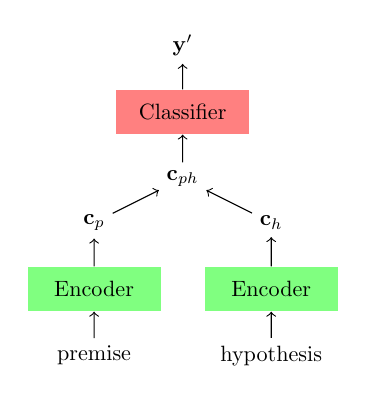
\begin{tikzpicture}[scale=0.8, every node/.style={scale=0.8}]
	\tikzstyle{block} = [rectangle, minimum width=6em,minimum height=2em]
	\node[](p)at (0,8em){$\mathbf{y}'$};
	\node[block,fill=red!50](classifier)at (0,5em){Classifier};
	\node[](chp)at (0,2em){$\mathbf{c}_{ph}$};
	\node[](cp)at (-4em,0){$\mathbf{c}_{p}$};
	\node[](ch)at (4em,0){$\mathbf{c}_{h}$};
	\node[block,fill=green!50]at (-4em,-3em)(encoder-p){Encoder};
	\node[block,fill=green!50]at (4em,-3em)(encoder-h){Encoder};
	\node[](premise)at (-4em,-6em){premise};
	\node[](hypo)at (4em, -6em){hypothesis};
	\path[->] (classifier) edge (p)
	(premise) edge (encoder-p)
	(hypo) edge (encoder-h)
	(encoder-p) edge (cp)
	(encoder-h) edge (ch)
	(cp) edge (chp)
	(ch) edge (chp)
	(chp) edge (classifier);
	\end{tikzpicture}
	\caption{Sentence entailment model, a shared encoder (green) encodes premise and hypothesis into fixed context vector $\mathbf{c}_{p}$ and $\mathbf{c}_{h}$, and then produce the intermediate vector $\mathbf{c}_{ph}$, before give prediction $\mathbf{y}'$.}
\end{figure*}
\subsection{Machine Translation}
We use the standard seq2seq model to solve this task, but note that the encoder is initialised with our pretrained RNN encoder. 
At testing time, the performance of machine translation is measured by bilingual evaluation understudy (BLEU) score\cite{papineni2002bleu}, one of the common and cheap evaluation techniques used in machine translation.\\\\
The BLEU score is calculated as follow 
\[ w_{n} = \frac{1}{N}\]
\[p_{n} = \frac{\text{numbers of matched n-gram}}{\text{total numbers of n-gram in reference}}\]
\begin{equation}
\text{BLEU Score} = \exp\{\min(1-\frac{r}{c}, 0)\} (\prod_{n=1}^{N}p_{n})^{w_{n}}
\end{equation}
Where $N$ is the size of n-gram up to, $p_{n}$ is known as n-gram precision between candidate and reference sentence, $r,c$ are the length of reference and candidate sentences, $w_{n}, p_{n}$ is the weight and precision of $n$th gram. Here we show an example of BLEU score calculation with $N = 4$.
\begin{figure}[h]
	\centering
	\includegraphics[width=0.7\linewidth]{BLEU}
	\caption{An example of BLEU score n-gram match}
	\label{fig:BLEU}
\end{figure}
\begin{table}[H]
	\begin{center}
		\begin{tabular}{|c|c|c|}
			\hline
			Metrics & Candidate One & Candidate Two \\
			\hline
			1-gram precision $(p_{1})$ & $3/6$ & $6/6$ \\
			\hline
			2-gram precision $(p_{2})$ & $1/5$ & $4/5$ \\
			\hline
			3-gram precision $(p_{3})$& $0/4$ & $2/4$ \\
			\hline
			4-gram precision $(p_{4})$& $0/3$ & $1/3$ \\
			\hline
			BLUE Score &  0 & 0.51 \\
			\hline
		\end{tabular}
	\end{center}
	\caption{BLEU Score example}
	\label{BLUE table}
\end{table}


